\subsection{Preventivo fase di collaudo}

\subsubsection{Divisione oraria}
La seguente tabella rappresenta la distribuzione oraria dei ruoli per ogni componente del gruppo:
{

	\rowcolors{2}{\evenRowColor}{\oddRowColor}
\renewcommand{\arraystretch}{2}
\begin{longtable}[h!] { C{3.5cm} C{1cm} C{1cm} C{1cm} C{1cm} C{1cm} C{1cm} C{2cm}}
\caption{Tabella della divisione oraria della fase di collaudo}	\\
\rowcolor{\primaryColor}

\textcolor{\secondaryColor}{\textbf{Membro del gruppo}} & 
\textcolor{\secondaryColor}{\textbf{RE}} & 
\textcolor{\secondaryColor}{\textbf{AM}} & 
\textcolor{\secondaryColor}{\textbf{AN}} & 
\textcolor{\secondaryColor}{\textbf{PT}} & 
\textcolor{\secondaryColor}{\textbf{PR}} & 
\textcolor{\secondaryColor}{\textbf{VE}} & 
\textcolor{\secondaryColor}{\textbf{Ore complessive}}\\	
\endhead

\AW{}                     &  - &  5 &  - & 10 & - & 10 & 25 \\
\AT{}                     &  - &  - &  5 & 5 & 7 & 8 & 25 \\
\AD{}                     &  - &  - &  - & - & 7 & 11 & 18 \\
\EC{}                     &  - &  10 &  - & - & 5 & 7 & 22 \\
\EM{}                     &  - &  - &  - & - & 10 & 12 & 22 \\
\FP{}                     & 10 & - &  - & - & 7 & 5 & 22 \\
\GG{}                     &  - &  - &  - & 5 & 7 & 10 & 22 \\
\textbf{Ore totali ruolo} & 10 & 15 & 5 & 20 & 43 & 63 & 156 \\

\end{longtable}
}


La suddivisione delle ore preventivate per ciascun componente del gruppo, a seconda del ruolo, viene rappresentata nel seguente istogramma:\\
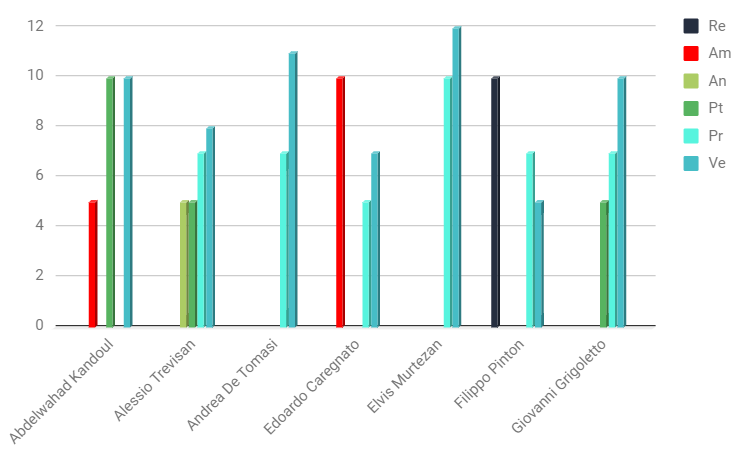
\includegraphics[width=1\textwidth]{./src/Preventivo/src/img/IstoValidazione.png}

%\begin{center}
%	\pgfplotsset{width=15.4cm, height=8.5cm}
%	\begin{tikzpicture}
%		\begin{axis}[
%			ybar stacked,
%			bar width=20pt,
%			legend style={
%				at={(0.5,-0.15)},
%				anchor=north,
%				legend columns=-1
%			},
%			symbolic x coords={Abdelwahad, Alessio, Andrea, Edoardo, Elvis, Filippo, Giovanni},
%			xtick=data
%		]
%			\legend{Responsabile, Amministratore, Analista, Progettista, Programmatore, Verificatore}
			% Responsabile
%			\addplot [ybar, fill=blue] coordinates {\ColonnaIstogramma{0}{0}{0}{0}{0}{10}{0}};
			% Amministratore
%			\addplot [ybar, fill=yellow] coordinates {\ColonnaIstogramma{5}{0}{0}{10}{0}{0}{0}};
			% Analista
%			\addplot [ybar, fill=red] coordinates {\ColonnaIstogramma{0}{5}{0}{0}{0}{0}{0}};
			% Progettista
%			\addplot [ybar, fill=green] coordinates {\ColonnaIstogramma{10}{5}{0}{0}{0}{0}{5}};
			% Programmatore
%			\addplot [ybar, fill=pink] coordinates {\ColonnaIstogramma{0}{7}{7}{5}{10}{7}{7}};
			% Verificatore
%			\addplot [ybar, fill=orange] coordinates {\ColonnaIstogramma{10}{8}{11}{7}{12}{5}{10}};
%		\end{axis}
%	\end{tikzpicture}
%\end{center}

\clearpage
% \subsubsection{Ore e costi degli incrementi}
% La seguente tabella rappresenta la distribuzione delle ore investite durante il periodo in cui vengono svolti gli incrementi e il corrispondente costo in euro.


% {
% \rowcolors{2}{\evenRowColor}{\oddRowColor}
% \renewcommand{\arraystretch}{1.65}
% \centering
% \begin{longtable}{ C{2.1cm} C{2.7cm} C{3cm} C{3cm} C{3.3cm} }
% \caption{Tabella del costo risultante di ogni incremento}\\
% \rowcolor{\primaryColor}
% \textcolor{\secondaryColor}{\textbf{Incremento}} & 
% \textcolor{\secondaryColor}{\textbf{Ore progettista}} &
% \textcolor{\secondaryColor}{\textbf{Ore programmatore}}&
% \textcolor{\secondaryColor}{\textbf{Ore verificatore}}&
% \textcolor{\secondaryColor}{\textbf{Costo totale incremento (in \euro{})}}\\
% \endhead



% x & x & x & x & x \\
% x & x & x & x & x \\
% x & x & x & x & x \\
% x & x & x & x & x \\


% \end{longtable}
% }
\subsubsection{Costo risultante}
La seguente tabella rappresenta le ore totali investite ed il corrispondente costo in euro per ogni ruolo:
{
\rowcolors{2}{\evenRowColor}{\oddRowColor}
\renewcommand{\arraystretch}{2}
\begin{longtable}{ C{3cm} C{2cm} C{4cm}}
\caption{Tabella del costo risultante di Collaudo}\\
\rowcolor{\primaryColor}

\textcolor{\secondaryColor}{\textbf{Ruolo}} & 
\textcolor{\secondaryColor}{\textbf{Totale ore}} & 
\textcolor{\secondaryColor}{\textbf{Costo ruolo (in \euro{})}}\\	
\endhead
        
Responsabile    &  10 & 300 \\
Amministratore  &  15 & 300 \\
Analista        &  5 & 125 \\
Progettista     &  20 & 440 \\
Programmatore   &  43 & 645 \\
Verificatore    &  63 & 945 \\
\textbf{Totale} & 156 & 2755 \\
	
\end{longtable}
}

\vskip 30pt %spazio verticale
\newpage
La quantità di ore totali per ciascun ruolo viene rappresentata nel seguente aerogramma:\\
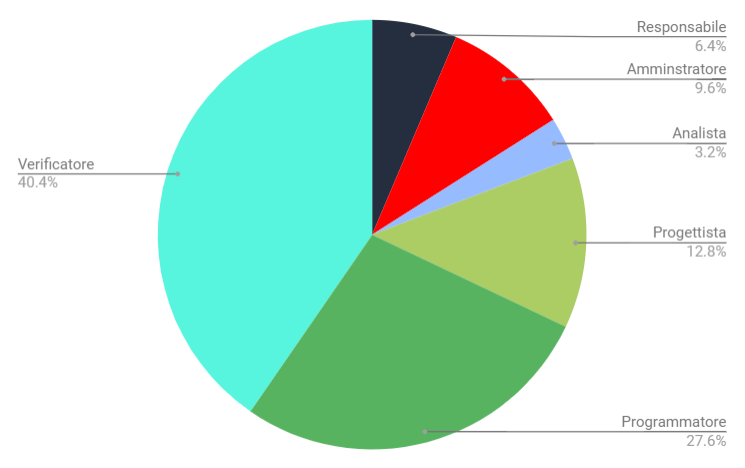
\includegraphics[width=1\textwidth]{./src/Preventivo/src/img/TortaValidazione.png}
%\begin{center}
%	\begin{tikzpicture}
%		\pie[rotate = 180, color={blue, yellow, red, green, pink, orange}] {
%			6/Responsabile,
%			10/Amministratore,
%			3/Analista,
%			13/Progettista,
%			27/Programmatore,
%			41/Verificatore
%		}
%	\end{tikzpicture}
%\end{center}
